\chapter{Theoretical Background}

\lettrine[
	nindent=0em, findent=0.5em, loversize=-0.12, lines=5
]{\initfamily{D}}{\bfseries\color{Blue}eep learning}\index{Deep learning},
\emph{a class of \gls{ml}\index{Machine learning} algorithms based on
\glspl{nn}}, has revolutionized the way we tackle a problem from a \gls{ml}
perspective and is one if not the most important factor for recent \gls{ml}
achievements. Solving complex tasks such image classification\index{Image
classification} or language translation\index{Language translation}, that for
years have bedevilled traditional \gls{ml} algorithms, constitutes the signature
of \gls{dl}. Admittedly, \emph{the advent of a deep
\gls{cnn}\index{Convolutional neural network}}, the AlexNet \parencite{alexnet}
on September 30 of 2012, signified the ``modern birthday'' of this field. On
this day, AlexNet\index{AlexNet} not only won the ImageNet \parencite{Deng_2009}
\gls{ilsvrc}, but dominated it, achieving a top-5 accuracy\index{Top-5 accuracy}
of \SI{85}{\percent}, surpassing the runner-up which achieved a top-5 accuracy
of \SI{75}{\percent}.  AlexNet showed that \glspl{nn} are not merely a
pipe-dream, but they can be applied in real-world problems. It is worth to
notice that ideas of \glspl{nn} trace back to 1943, but it was until recently
that these ideas got materialized. The reason for this recent breakthrough of
\gls{dl} (and \gls{ml}) is twofold. First, the availability of large
datasets\index{Dataset}---the era of big data\index{Big data}---such as
ImagNet\index{ImageNet}. Second, the increase in computational power, mainly of
\acrshortpl{gpu} for \gls{dl}, accelerating the training of deep \glspl{nn} and
traditional \gls{ml} algorithms.

\section{Machine Learning Preliminaries}

Since \gls{dl} is a subfield of \gls{ml}, it is necessary to familiarize with
the later before diving into the former. In this section, the minimum
theoretical background and jargon of \gls{ml} is presented. \Acrlong{ml} can be
defined as \emph{``the science and (art) of programming computers so they can
learn from the data''} \parencite{ml}. A more technical definition is the following:

\begin{definition}[name={Machine learning, \cite{mitchell}}]
	A computer program is said to learn from experience\index{Experience}
	\textbf{E} with respect to some class of tasks\index{Task} \textbf{T} and some
	performance measure \textbf{P}\index{Performance measure}, if its
	performance on \textbf{T}, as measured by \textbf{P}, improves with
	experience \textbf{E}.
\end{definition}

For instance, a computer program\index{Spam filter} that classifies emails into
spam and non-spam (the task \textbf{T}), can improve its accuracy, i.e. the
percentage of correctly classified emails (the performance \textbf{P}), through
examples of spam and non-spam emails (the experience \textbf{E}). But in order
to take advantage of the experience aka \emph{data}\index{Data}, it must be
written in such a way that \emph{adapts to the patterns in the data}. Certainly,
a \emph{traditional spam filter can not learn from experience}, since the latter
does not affect the classification rules of the former and as such, its
performance. For a traditional spam filter to adapt to new patterns and perform
better, it must change its hard-wired rules, but by then it will be a different
program. In contrast, a \emph{\gls{ml}-based filter can adapt to new patterns,
simply because it has been programmed to do so}. In other words, \emph{in
traditional programming\index{Traditional programming} we write rules for
solving \textbf{T} whereas \textbf{in \gls{ml} we write rules to learn the
rules} for solving \textbf{T}}. This subtle but essential difference is what
gives \gls{ml} algorithms the ability to take advantage of the data.

\subsection{Learning paradigms}
\label{subsec:paradigms}

Depending on the type of experience they are allowed to have during their
\emph{training phase} \parencite{deeplearning}, \gls{ml} approaches are divided
into three main \emph{learning paradigms}\index{Learning paradigms}:
\emph{\textbf{unsupervised learning}\index{Unsupervised learning},
\textbf{supervised learning}\index{Supervised learning} and
\textbf{reinforcement learning}\index{Reinforcement learning}}. The following
definitions are not by any means formal, but merely serve as an intuitive
description of the different paradigms.

\begin{definition}[name=Unsupervised learning]
	The experience comes in the form $\dtrain = \{\vcx_i\}$, where $\vcx_i \sim
	p(\vcx)$ is the input\index{Input} of the $i$-th training
	instance\index{Training instance}. In this paradigm we are interested in
	learning useful properties of the underlying structure captured by
	$p(\vcx)$.
\end{definition}

For example, suppose we are interested in generating images that look like
Picasso paintings. In this case, the input is just the pixel values, i.e.  $\vcx
\in \mathbb{R}^{W \times H \times 3}$. The latter follow a distribution
$p(\vcx)$, so all we have to do is to train an unsupervised learning algorithm
with many Picasso paintings to get a \emph{model}, that is $\hat{p}(\vcx)$.
Assuming the estimation of the original distribution is good enough, new
realistically looking paintings (with respect to original Picasso paintings) can
be ``drawn'' by just sampling from $\hat{p}(\vcx)$. In the ML parlance, inputs
are also called \emph{features, predictors or
descriptors}\index{Feature}\index{Descriptor}\index{Predictor}.

\begin{definition}[name=Supervised learning]
	The experience comes in the form $\dtrain = \{(\vcx_i, \vcy_i)\}$, where
	$(\vcx_i, \vcy_i) \sim p(\vcx, \vcy)$ and $\vcy_i$ is the
	output\index{Output} aka label\index{Label} of the $i$-th training instance.
	In this paradigm we are usually interested in learning a function $f \colon
	X \to Y$.
\end{definition}

\textbf{ADD figure regression and classification}

This paradigm comes mainly under two flavors: \emph{regression\index{Regression}
and classification\index{Classification}.} In regression the interest is in
predicting a continuous value given an input, i.e.  $y \in \mathbb{R}$, such as
a molecular property given a mathematical representation of a molecule. In
classification, the interest is to predict in which of $k$ classes an input
belongs to, i.e. $y \in \{1, \ldots, k\}$, such as predicting the breed of a dog
image given the raw pixel values of the image. The term ``supervised'' is coined
due to the ``human supervision'' the algorithm receives during its training
phase, through the presence of the correct answer (the label) in the experience.
In a sense, in this paradigm we ``teach'' the learning algorithm aka
\emph{learner}. It should be emphasized that the label is not constrained to be
single-valued, but can also be multi-valued. In this case, one talks about
\emph{multi-label regression\index{Multi-label regression} or
classification\index{Multi-label classification}} \parencite{Read_2009}.

A more exotic form of supervised learning is \emph{conditional generative
modelling}\index{Conditional generative modelling}, where the interest is in
estimating $p(\vcx \mid \vcy)$. For example, one may want to build a model that
generates images of a specific category or a \emph{model that designs
molecules/materials with tailored properties} \parencite{Kim2018, Yao2021,
Gebauer2022}. This is one approach of how \gls{ml} can tackle the \emph{inverse
design problem}\index{Inverse design} in chemistry.

\begin{definition}[Reinforcement learning]
	The experience comes from the interaction of the learner, called
	agent\index{Agent} in this context, with its environment. In other words,
	there is a feedback loop between the learner and its environment. In this
	paradigm we are interested in building an agent that can take suitable
	actions in a given situation.
\end{definition}

The agent observes its \emph{environment}, selects and performs \emph{actions}
and gets \emph{rewards or penalties} in return. The goal is to learn an optimal
strategy, called a \emph{policy}, that \emph{maximizes the long-term reward}
\parencite{ml}. A policy simply defines the action that the agent should
choose in a given situation. In contrast to supervised learning, where the
correct answers are provided to the learner, \emph{in reinforcement learning the
learner must find the optimal answers by trial and error}
\parencite{bishop2007}. Reinforcement learning techniques find application in
fields such as gaming (AlphaGo is a well known example), robotics, autonomous
driving and recently chemistry \parencite{li, Gow2022}. Since in the present
thesis only supervised learning techniques were employed, the remaining of this
chapter is devoted to this learning paradigm.

\subsection{Formulating the problem of supervised learning}

The general setting of supervised learning is as follows: we assume that there
is some relationship between $\vcx$ and $\vcy$:
\begin{equation}
	\label{eq:supervised}
	\vcy = f(\vcx) + \vc{\epsilon}
\end{equation}
and we want to estimate $f$ from the data. The function $f$ represents the
\emph{systematic information} that $\vcx$ gives about $\vcy$ while
$\vc{\epsilon}$ is a random \emph{error term}\index{Error term} independent of
$\vcx$ and with zero mean. More formally, we have an input space $X$, an output
space $Y$ and we are interested in learning a function $\hat{h} \colon X \to Y$,
called the \emph{hypothesis}\index{Hypothesis}, which produces
an output $\vcy \in Y$ given an input $\vcx \in X$. At our disposal we have a
collection of input-output pairs $(\vcx_i, \vcy_i)$, forming the \emph{training
set}\index{Training set} $\dtrain$, with the pairs drawn \acrshort{iid} from
$p(\vcx, \vcy)$.

Ideally, we would like to learn a hypothesis that minimizes the
\emph{generalization error or loss}\index{Generalization
error}\index{Generalization loss}:
\begin{equation}
	\label{eq:generalization_loss}
	\loss \coloneqq \int_{X \times Y} \ell(h(\vcx), \vcy) p(\vcx, \vcy) d\vcx d\vcy
\end{equation}
that is, the expected value of some \emph{loss function}\index{Loss function}
$\ell$ over all possible input-output pairs. A loss function just measures the
discrepancy of the prediction $h(\vcx) = \hat{\vcy}$ from the true value $\vcy$
and as such, the best hypothesis is the one that minimizes this integral.
Obviously, it is impossible to evaluate the integral in Equation
\ref{eq:generalization_loss}, since we don't have access to infinite data.

The idea is to use the \emph{training error or loss}\index{Training
error}\index{Training loss}:
\begin{equation}
	\label{eq:training_loss}
	\loss_\text{train} \coloneqq \frac{1}{\lvert \dtrain \rvert} \sum_{i \in \dtrain}
	\ell(h(\vcx_i), \vcy_i)
\end{equation}
as an approximation for the generalization loss, and \emph{choose the hypothesis
that minimizes the training loss}, a principle known as \emph{empirical risk
minimization}\index{Empirical risk minimization}. In other words, to get a
hypothesis aka \emph{model} $\mcl{M}$\index{Model} from the data, we need to
solve the following optimization problem:
\begin{equation}
	\label{eq:problem}
	\hat{h} \gets \argmin_{h \in \mcl{H}} \ltrain
\end{equation}
which is achieved, by just feeding the training data into the learning
algorithm $\mcl{A}$\index{Learning algorithm}:
\begin{equation}
	\label{eq:learner}
	\mcl{M} \gets \mcl{A}(\dtrain)
\end{equation}

\subsection{Components of a learning algorithm}

By breaking down Equation \ref{eq:problem}, i.e. the optimization problem the
learner needs to solve, the components of a learner can be revealed. The latter
is comprised of the following three ``orthogonal'' components: a
\emph{\textbf{hypothesis space}}\index{Hypothesis space}, a \emph{\textbf{loss
function}} and an \emph{\textbf{optimizer}}. We now look into each of them
individually and describe the contribution of each one to the solution of the
optimization problem. For the ease of notation and clarity, in the remaining of
this chapter we will stick to examples from simple (single-valued) regression
and binary classification.

\begin{definition}[Hypothesis space]
	The set of hypotheses (functions), denoted as $\mcl{H}$, from which the
	learner is allowed to pick the solution of Equation \ref{eq:problem}.
\end{definition}

A simple example of a hypothesis space, is the one used in univariate
\emph{linear regression}\index{Linear regression}:
\begin{equation}
	\label{eq:linear}
	\hat{y} = \beta_0 + \beta x
\end{equation}
where $\mcl{H}$ contains all lines (or hyperplanes in the multivariate case)
defined by Equation \ref{eq:linear}. Of course, one can get \emph{a
more expressive} hypothesis space, by including polynomial terms, e.g.:
\begin{equation}
	\label{eq:polynomial}
	\hat{y} = \beta_0 + \beta_1 x + \beta_2 x^2
\end{equation}
The more expressive the hypothesis space, the larger the
\emph{\textbf{representational capacity}}\index{Representational capacity} of
the learning algorithm. For a formal definition of representational capacity,
the interested reader can look at \emph{Vapnik-Chervonenkis
Dimension}\index{Vapnik-Chervonenkis dimension} \parencite{statlearn}.

\begin{definition}[Loss function]
	A function that maps a prediction into a real number, which intuitively
	represents the quality of a candidate hypothesis.
\end{definition}

For example, a typical loss function used in regression is the \emph{squared
loss}\index{Squared loss}:
\begin{equation}
	\label{eq:squared_loss}
	\ell(\hat{y}, y) \coloneqq (\hat{y} - y)^2
\end{equation}
where $y, \hat{y} \in \mathbb{R}$. A typical loss function for binary
classification is the \emph{binary cross entropy
loss}\index{Binary cross entropy loss}:
\begin{equation}
	\label{eq:cross_entropy}
	\ell(\hat{y}, y) \coloneqq y \cdot \log (\hat{y})
	+ (1 - y) \cdot \log (1 - \hat{y})
\end{equation}
where $y \in \{0, 1\}$, indicating the correct class, and $\hat{y} \in [0, 1]$
which corresponds to the predicted probability for class-$1$. Notice that in
both cases the loss is minimum when the prediction is equal to the ground truth.
For the cross entropy loss, if $y=1$ is the correct class, then the model must
predict $\hat{y}=1$ for the loss to be minimized.

Usually, we are not only penalizing a hypothesis for its mispredictions, but
also for its \emph{complexity}. This is done in purpose, since a learner with a
\emph{very rich hypothesis space} can easily memorize the training set but fail
to generalize well to new unseen examples. \emph{Every modification that is made
to a learner in order to reduce its generalization loss but not its training
loss, is called \textbf{regularization}}\index{Regularization} \parencite{deeplearning}.

A common---but not the only---way to achieve that, is by including another
penalty term called \emph{regularization term or
regularizer}\index{Regularizer}, denoted as $\mcl{R}$, in Equation
\ref{eq:training_loss}:
\begin{equation}
	\label{eq:regularization}
	\loss_\text{train} \coloneqq \frac{1}{\lvert \dtrain \rvert} \sum_{i \in \dtrain}
	\ell(h(\vcx_i), \vcy_i)
	+
	\lambda \mcl{R}
\end{equation}
The $\lambda$ factor controls the strength of regularization and it is an
\emph{\textbf{hyperparameter}}\index{Hyperparameter}, i.e. a parameter that is
not learned during training but \emph{whose value is used to control the
training phase.} In order to see how $\lambda$ penalizes model complexity,
assume we perform univariate polynomial regression\index{Polynomial regression}
of degree $k$:
\begin{equation}
	\hat{y} = \beta_0 + \sum_{i=1}^k \beta_i x^i
\end{equation}
combining \gls{msl}\index{Mean squared loss} and \emph{Lasso
regularization}\index{Lasso} as training loss:
\begin{equation}
	\label{eq:lasso}
	\loss_\text{train} = \frac{1}{\lvert \dtrain \rvert} \sum_{i \in \dtrain}
	\ell(\hat{y}_i - y_i)^2
	+
	\lambda \sum_{i=1}^k \lvert \beta_i \rvert
\end{equation}
Lets apply a very strong regularization by setting $\lambda \to \infty$ (in
practice we set $\lambda$ to a very large value) and observe what happens to the
\emph{weights}\index{Weights} $\beta_i$. By setting $\lambda \to
\infty$, the regularization term dominates the \gls{msl} and as such, the only
way to minimize the training loss is by setting $\beta_i \to 0$. This leave us
with a very simple model---only the \emph{bias}\index{Bias} $\beta_0$
survives---which always predicts the mean value of $y$ in the training set.

Applying a regularizer\index{Regularizer}, is also useful when we need to select
between two (or more) competing hypotheses that are equally good. For example,
assuming two hypotheses achieve the same (unregularized) training loss, the
inclusion of a regularization term help us decide between the two, \emph{by
favoring the simplest one}. This is reminiscent of the \emph{Occam's razor aka
principle of parsimony}, which advocates that between two competing theories
with equal explanatory power, one should prefer the one with the fewest
assumptions.

\begin{definition}[Optimizer]
	An algorithm that searches through $\mcl{H}$ for the solution of Equation
	\ref{eq:problem}.
\end{definition}

Having defined the set of candidate models (the hypothesis space) and a measure
that quantifies the quality of a given model (the loss function), all that is
remaining is a tool to scan the hypothesis space and pick the model that
minimizes the training loss (the optimizer). A naive approach is to check all
hypotheses in $\mcl{H}$ and then pick the one that achieves the lowest training
loss. This approach can work if $\mcl{H}$ is finite, but obviously doesn't scale
in the general case where $\mcl{H}$ is infinite\footnote{It is not
uncommon for $\mcl{H}$ to be infinite. Even for simple learners like linear
regression $\mcl{H}$ is infinite, since there infinite lines defined by Equation
\ref{eq:linear}.}. More efficient approaches are needed if we are aiming to solve
Equation \ref{eq:problem} in finite time.

One optimizer that is frequently used in \gls{ml} and is the precursor of more
refined ones, is \emph{\textbf{gradient descent}}\index{Gradient descent}. With
this method, the exploration of hypothesis space\footnote{We have implicitly
assumed that $\mcl{H}$ can be parameterized, i.e. $\mcl{H} = \{h(\vcx;\vcth)
\mid \vcth \in \Theta\}$, where $\Theta$ denotes the parameter space, the set of
all values the parameter $\vcth$ can take. This allows us to write the training
loss as function of model parameters and optimize them with gradient descent.}
involves the following steps:

\begin{algorithm}[H]
	Random initialization of $\vcth$\;
	\While{stopping criterion not met}{
		$\vcth \gets \vcth - \eta \nabla_{\vcth}\ltrain(\vcth)$\; 
	}
	\caption{Gradient descent}
	\label{algo:gd}
\end{algorithm}

\noindent where $\eta$ is a small number called the \emph{learning
rate}\index{Learning rate}. Gradient descent is based on the idea that
if a multivariate function is defined and differentiable at a point $\vcx$, then
$f(\vcx)$ \emph{decreases fastest if one takes a small step from $\vcx$ in the
direction of negative gradient at $\vcx$, $-\nabla f(\vcx)$}. The motivation
becomes clear if we look at the differential of $f(\vcx)$ in direction $\vc{u}$:
\begin{equation}
	\label{eq:differential}
	f(\vcx + \delta \vc{u}) - f(\vcx) = \nabla f(\vcx) \cdot \delta \vc{u}
\end{equation}
Equation \ref{eq:differential} says that this differential is
minimized\footnote{The right hand side of Equation \ref{eq:differential} is a
dot product.} when $\delta \vc{u}$ is anti-parallel to $\nabla f(\vcx)$ and that
is why we subtract the gradient in Algorithm \ref{algo:gd}. The fact that
Equation \ref{eq:differential} holds only locally (magnitude of $\delta \vc{u}$
must be small) explains why $\eta$ must be a small number. It should be added
that gradient descent can be trapped to (potential) local minima of the training
loss and therefore fail to solve Equation \ref{eq:problem}. As it will be
discussed later, this is not a problem, because \emph{the ultimate purpose is to
find a hypothesis that generalizes well, not necessarily the one that minimizes
the training loss}\footnote{Remember we use the training loss (see Equation
\ref{eq:training_loss}) as a proxy for the generalization loss (see Equation
\ref{eq:generalization_loss}).}. Optimizers are discussed in further detail in
the next section.

Before moving on, it is worth to add that both the regularization and the
optimizer can effect the ``true'' or \emph{\textbf{effective
capacity}}\index{Effective capacity} \parencite{deeplearning} of the learner,
\emph{which might be less than the representational
capacity\index{Representational capacity} of the hypothesis space}. For example
a regularizer penalizes the complexity of an hypothesis, effectively
``shrinking'' the representational capacity of the hypothesis space. The effect
of the optimizer can be understood by looking on its contribution to the
solution of Equation \ref{eq:problem}. As described previously, the optimizer
searches through the hypothesis space. If this ``journey'' is not long enough,
then this ``journey'' is practically equivalent to a long ``journey'' in a
shortened version of the original hypothesis space. In the rest of this chapter,
by the term \emph{complexity\index{Complexity} or capacity\index{Capacity} of a
learner, we mean its effective capacity, which is affected by all its three
components}.

%\begin{figure}
%	\centering
%	\begin{tikzpicture}
%		\begin{axis}[ width=0.8\textwidth, custom axis, domain=0:2,
%		xlabel=Complexity | $\Omega$, ylabel=Error | $\mathcal{E}$, samples=50,
%		ymin=0, ymax=2, grid=none, ticks=none ]
%			\addplot+ [no markers] {1/(x+0.3)-0.2}; % Bias^2
%			\addlegendentry{Bias$^2$};
%			\addplot+ [no markers] {0.12*e^(1.40*x)}; % Variance
%			\addlegendentry{Variance};
%			\addplot+ [no markers] {3*(x-2)*x+3.8}; % Total error
%			\addlegendentry{Total error};
%			\draw[dotted, -Diamond] (1, 0) -- (1, 0.83) node[
%				above, yshift=0.2cm
%			] {$\argmin_{\Omega} \mathcal{E}$};
%		\end{axis}
%	\end{tikzpicture}
%	\caption{The bias-variance tradeoff in \LaTeX.}
%\end{figure}
%
%\begin{figure}
%	\begin{subfigure}{0.5\textwidth}
%		\centering
%		\begin{tikzpicture}%[trim axis left, trim axis right]
%			\begin{axis}[
%					custom axis, no markers, ticks=none,
%					xmin=0, xmax=3.5, domain=0:3.5, grid=none,
%					ymin=0, ymax=1.2, clip mode=individual,
%					xlabel=Number of training samples, ylabel=Accuracy,
%					axis background/.style={
%						shade,
%						right color=gray,
%						left color=white,
%						middle color=Blue!90,
%					}
%				]
%				%\shadedraw[
%				%	left color=Peach!40,
%				%	right color=Blue!50,
%				%	middle color=Blue!20,
%				%	black
%				%] (0, 0) rectangle (3.5, 1.2);
%				\addplot+[ultra thick] {divide(25*x, 2+25*x)*0.6};
%				\addlegendentry{Test accuracy};
%				\addplot+[ultra thick] {1 - 0.59*divide(25*x, 2+25*x)*0.6};
%				\addlegendentry{Training accuracy};
%				\addplot+ [black, dashed] {1};
%				\node at (-0.29, 1) {100\%};
%			\end{axis}
%		\end{tikzpicture}
%	\end{subfigure}
%	\begin{subfigure}{0.5\textwidth}
%		\centering
%		\begin{tikzpicture}%[trim axis left, trim axis right]
%			\begin{axis}[
%					custom axis, no markers, ticks=none,
%					xmin=0, xmax=3.5, domain=0:3.5,
%					ymin=0, ymax=1.2, clip mode=individual,
%					xlabel=Number of training samples, ylabel=Accuracy,
%				]
%				\shadedraw[
%					left color=Peach!40,
%					right color=Blue!50,
%					middle color=Peach!20,
%					black
%				] (0, 0) rectangle (3.5, 1.2);
%				\addplot+[ultra thick] {divide(25*x, 11+25*x)*0.97};
%				\addlegendentry{Test accuracy};
%				\addplot+[ultra thick] {1 - 0.1*divide(25*x, 11+25*x)*0.97};
%				\addlegendentry{Training accuracy};
%				\addplot+[black, dashed] {1};
%				\node at (-0.29, 1) {100\%};
%			\end{axis}
%		\end{tikzpicture}
%	\end{subfigure}
%\end{figure}

%\begin{definition}[Overfitting]
%	Add some text!
%\end{definition}
%
%\begin{definition}[Underfitting]
%	Add some text!
%\end{definition}
%
%\begin{theorem}[No free lunch]
%	Add some text!
%\end{theorem}
%
%\begin{theorem}[Bias-variance tradeoff]
%\end{theorem}
%
%\begin{proof}
%	This is mhy proof.
%\end{proof}
%
%\section{Deep Learning}
%
%\section{Training Neural Networks}
%
%\begin{algorithm}[H]
%	\KwIn{
%		$\dtrain$, loss function $\ell$,
%		model parameters $\vcth$, learning rate
%		$\eta$, batch size $\lvert\mcl{B}\rvert$
%	}
%	\KwOut{Estimated parameters $\hvcth$}
%	\BlankLine
%	$\vcth \gets$ random initialization\;
%	\While{stopping criterion not met}{
%		$\mcl{B} \gets$ sample $\lvert\mcl{B}\rvert$ datapoints from $\dtrain$\;
%		$\gloss \gets \frac{1}{\lvert\mcl{B}\rvert} \sum_{i \in \mcl{B}}
%		\nabla_{\vcth}\ell_i(\vcth)$\;
%		$\vcth \gets \vcth - \eta\gloss$\;
%	}
%	$\hvcth \gets \vcth$\;
%	\Return{$\hvcth$}
%	\caption{Batch\index{Batch gradient descent}, mini-batch\index{Mini-batch
%	gradient descent} and stochastic gradient descent\index{Stochastic gradient
%	descent} algorithms}
%\end{algorithm}
%
%\begin{algorithm}[H]
%	\KwIn{Model parameters $\vcth$, momentum $\beta$, learning rate $\eta$}
%	\KwOut{Estimated parameters $\hvcth$}
%	\BlankLine
%	$\vcth \gets$ random initialization\;
%	\While{stopping criterion not met}{
%		$\vc{m} \gets \beta\vc{m} - \gloss$\;
%		$\vcth \gets \vcth + \vc{m}$\;
%	}
%	$\hvcth \gets \vcth$\;
%	\Return{$\hvcth$}
%	\caption{Momentum\index{Momentum} algorithm, citation}
%	\label{algo:momentum}
%\end{algorithm}
%
%\begin{algorithm}[H]
%	\KwIn{Model parameters $\vcth$, momentum $\beta$, learning rate $\eta$}
%	\KwOut{Estimated parameters $\hvcth$}
%	\BlankLine
%	$\vcth \gets$ random initialization\;
%	\While{stopping criterion not met}{
%		$\vc{m} \gets \beta\vc{m} -
%		\eta\nabla_{\vcth}\loss(\vcth + \beta\vc{m})$\;
%		$\vcth \gets \vcth + \vc{m}$\;
%	}
%	$\hvcth \gets \vcth$\;
%	\Return{$\hvcth$}
%	\caption{Nesterov momentum\index{Nesterov momentum} algorithm, citation}
%	\label{algo:nesterov}
%\end{algorithm}
%
%\begin{algorithm}[H]
%	\KwIn{
%		Model parameters $\vcth$, momentum $\beta$, learning rate $\eta$,
%		smoothing term $\epsilon$
%	}
%	\KwOut{Estimated parameters $\hvcth$}
%	\BlankLine
%	$\vcth \gets$ random initialization\;
%	\While{stopping criterion not met}{
%		$\vc{s} \gets \vc{s} + \gloss \odot \gloss$\;
%		$\vcth \gets \vcth - \eta\gloss \oslash \sqrt{\vc{s} + \epsilon}$\;
%	}
%	$\hvcth \gets \vcth$\;
%	\Return{$\hvcth$}
%	\caption{AdaGrad\index{AdaGrad} algorithm, citation}
%	\label{algo:adagrad}
%\end{algorithm}
%
%\begin{algorithm}[H]
%	\KwIn{
%		Model parameters $\vcth$, decay rate $\beta$, learning rate $\eta$,
%		smoothing term $\epsilon$
%	}
%	\KwOut{Estimated parameters $\hvcth$}
%	\BlankLine
%	$\vcth \gets$ random initialization\;
%	\While{stopping criterion not met}{
%		$\vc{s} \gets \vc{s} + (1 - \beta) \gloss \odot \gloss$\;
%		$\vcth \gets \vcth - \eta\gloss \oslash \sqrt{\vc{s} + \epsilon}$\;
%	}
%	$\hvcth \gets \vcth$\;
%	\Return{$\hvcth$}
%	\caption{RMSProp\index{RMSProp} algorithm, citation}
%	\label{algo:rmsprop}
%\end{algorithm}
%
%\begin{algorithm}[H]
%	\KwIn{
%		Model parameters $\vcth$,
%		learning rate $\eta$, smoothing term $\epsilon$,
%		momentum decay $\beta_1$, scaling decay $\beta_2$
%	}
%	\KwOut{Estimated parameters $\hvcth$}
%	\BlankLine
%	$\vcth \gets$ random initialization\;
%	\While{stopping criterion not met}{
%		$\vc{m} \gets \beta_1\vc{m} - (1 - \beta_1) \gloss$\;
%		$\vc{s} \gets \beta_2\vc{s} + (1 - \beta_2) \gloss \odot \gloss$\;
%		$\vc{\widehat{m}} \gets \frac{\vc{m}}{1 - \beta_1^t}$\;
%		$\vc{\widehat{s}} \gets \frac{\vc{s}}{1 - \beta_2^t}$\;
%		$\vcth \gets \vcth + \eta\widehat{\vc{m}}
%		\oslash \sqrt{\vc{\widehat{s}} + \epsilon}$\;
%	}
%	$\hvcth \gets \vcth$\;
%	\Return{$\hvcth$}
%	\caption{Adam\index{Adam} algorithm, citation}
%	\label{algo:adam}
%\end{algorithm}
%
%\begin{algorithm}[H]
%	\KwIn{Computational graph $\mcl{G}$ where nodes $u_i$ follow a topological
%	ordering\footnote{Any ordering such that parents come before children.}}
%	\KwOut{Derivatives $\bar{u}_i$}
%	\BlankLine
%	\tcc{Forward pass}
%	\For{$i=1$ \KwTo $N$}{
%		Compute $u_i$ as a function of $\text{Pa}_\mcl{G}(u_i)$\;
%	}
%	$u_N = 1$\;
%	\tcc{Backward pass}
%	\For{$i=N-1$ \KwTo $1$}{
%		$\bar{u}_i =
%		\sum_{j \in \text{Ch}_\mcl{G}(u_i)} \bar{u}_j \pd{u_j}{u_i}$\;
%	}
%	\caption{Backpropagation\index{Backpropagation} algorithm, citation}
%	\label{algo:backpropagation}
%\end{algorithm}
%
%\begin{figure}
%	\centering
%	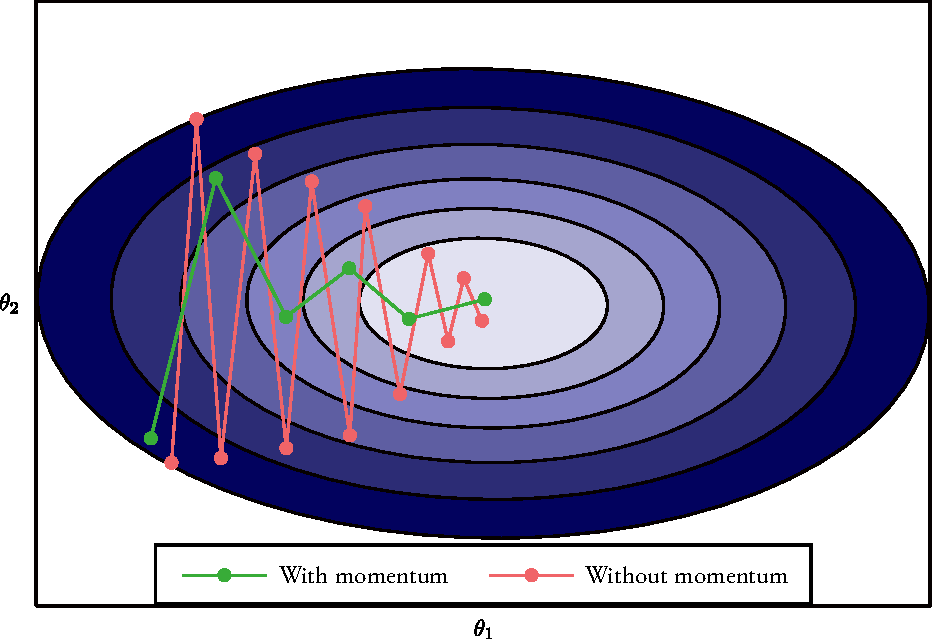
\includegraphics[width=\textwidth]{momentum.pdf}
%\end{figure}
%
%\begin{figure}
%	\centering
%	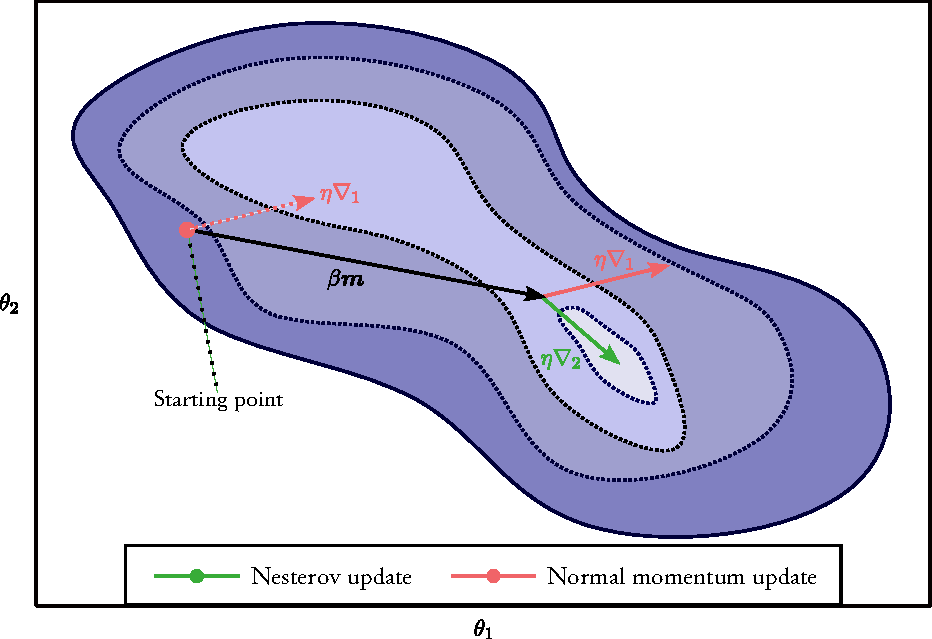
\includegraphics[width=\textwidth]{nesterov.pdf}
%\end{figure}


%\begin{figure}
%	\begin{subfigure}{0.49\textwidth}
%		\begin{tikzpicture}
%			\begin{axis}[custom axis, no markers, title=Foo]
%				\addplot {tanh(x)};
%				\addlegendentry {$\tanh(x)$};
%			\end{axis}
%		\end{tikzpicture}
%	\end{subfigure}
%	\hfill
%	\begin{subfigure}{0.49\textwidth}
%		\begin{tikzpicture}
%			\begin{axis}[custom axis, no markers, title=Foo bar]
%				\addplot {max(0, x)};
%			\end{axis}
%		\end{tikzpicture}
%	\end{subfigure}
%	\caption{Plots of some common activation functions.}
%\end{figure}
%
%\lipsum
%
%\begin{figure}
%	\centering
%	\begin{tikzpicture}
%		\pgfplotsset{width=0.8\textwidth}
%		\begin{axis}[
%				clip mode=individual, custom axis, domain=-8:8, ymin=0, ymax=10,
%				no markers, xlabel=$w$, ylabel=$\mathcal{L}(w)$, samples=500, grid=none
%			]
%			\draw[gray, fill=gray!30] (-2, 0) rectangle (2, 10);
%			\addplot {pow(x-2, 2)};
%			\addlegendentry{$\mathcal{L}_1$};
%			\addplot {pow(x, 2)};
%			\addlegendentry{$\mathcal{L}_2$};
%			\addplot {pow(x+2, 2)};
%			\addlegendentry{$\mathcal{L}_3$};
%			\addplot {pow(3*x, 2) + 2.667};
%			\addlegendentry{$\mathcal{L}_{\mathrm{T}}$};
%			%\node at (-2, -0.9) [font=\scriptsize] {$\min_i w_i$};
%			\node at (-2, -0.9)  {$\min_i w_i$};
%			%\node at (2, -0.9) [font=\scriptsize] {$\max_i w_i$};
%			\node at (2, -0.9)  {$\max_i w_i$};
%			\node at (0, 2.4) {$w^*$};
%			%\draw[dotted, -Diamond] (0, 0) -- (0, 2.1) node[above] {$w^*$};
%		\end{axis}
%	\end{tikzpicture}
%	\caption{Explaining why SGD works.}
%\end{figure}
%
%\lipsum
%
%
%\lipsum
%
%\begin{figure}
%	\begin{subfigure}{0.24\textwidth}
%		\centering
%		\begin{tikzpicture}[node distance=1.5cm, on grid, semithick]
%			\node[custom node] (1) {1};
%			\node[custom node, right of=1] (2) {2};
%			\node[custom node, above of=1] (3) {3}
%				edge (1);
%			\node[custom node, above of=2] (4) {4}
%				edge (2) edge (3);
%			\node[custom node, above of=3, xshift=0.75cm] {5}
%				edge (3) edge (4);
%		\end{tikzpicture}
%	\end{subfigure}
%	\begin{subfigure}{0.24\textwidth}
%		\centering
%		\begin{tikzpicture}[node distance=1.5cm, on grid, semithick]
%			\node[custom node] (1) {1};
%			\node[custom node, right of=1] (2) {2};
%			\node[custom node, above of=1] (3) {3}
%				edge [<-] (1);
%			\node[custom node, above of=2] (4) {4}
%				edge [<-] (2) edge [blue, <-] (3);
%			\node[custom node, above of=3, xshift=0.75cm] {5}
%				edge [blue, ->] (3) edge [blue, <-] (4);
%		\end{tikzpicture}
%	\end{subfigure}
%	\begin{subfigure}{0.24\textwidth}
%		\centering
%		\begin{tikzpicture}[node distance=1.5cm, on grid, semithick]
%			\node[custom node] (1) {1};
%			\node[custom node, right of=1] (2) {2};
%			\node[custom node, above of=1] (3) {3}
%				edge [<-] (1);
%			\node[custom node, above of=2] (4) {4}
%				edge [<-] (2) edge [blue, <-] (3);
%			\node[custom node, above of=3, xshift=0.75cm] {5}
%				edge [blue, <-] (3) edge [blue, <-] (4);
%		\end{tikzpicture}
%	\end{subfigure}
%	\begin{subfigure}{0.24\textwidth}
%		\centering
%		\begin{tikzpicture}[node distance=1.5cm, on grid, semithick]
%			\node[custom node] (x1) {$x_1$};
%			\node[custom node, right of=x1] (x2) {$x_2$};
%			\node[custom node, above of=x1] (h1) {$h_1$}
%				edge[<-] (x1) edge[<-] (x2);
%			\node[custom node, above of=x2] (h2) {$h_2$}
%				edge [<-] (x1) edge[<-] (x2);
%			\node[custom node, above of=h1, xshift=0.75cm] {$y$}
%				edge [<-] (h1) edge [<-] (h2);
%		\end{tikzpicture}
%	\end{subfigure}
%\end{figure}
%
%\lipsum
